\appendix

\section{Comparison between the PMV formulations with the \ac{pmvg}}\label{sec:comparison-between-the-pmv-formulations-with-the-two-node-model}
We compared how the results of the \ac{pmv} and \ac{pmv-ce} perform against the results of the \ac{pmvg}.
% SS provide more information why this was done
% Stefano Schiavon: Please provide more details of how these inputs were generated, within which ranges, etc.
Figure~\ref{fig:pmv_two_node_comparison} was generated by calculating the three \ac{pmv} values using the same combination of \num{10000} randomly generated sets inputs.
The \ac{pmv} and \ac{pmv-ce} were then plotted on the y-axis while the \ac{pmvg} value was on the x-axis.
The Figure also shows the \ac{lowess} curves that are used to visualize the prevailing data trend.
% Stefano Schiavon: Beside the visualization, can you discuss here also the quantitative results to support the conclusion?
The results of the \ac{pmv} model had a higher agreement than those obtained with the \ac{pmv-ce} model for \ac{pmvg} $\geq$ \qty{0.5}{\m\per\s}.
% Stefano Schiavon: This is unclear and cannot be deduced from the figure, from where does it come from? How can a PMV model be described by an air speed?
These results show the \ac{pmv-ce} is less similar to the \ac{pmvg} model than the \ac{pmv}, despite using it in the backend to calculate the cooling effect.
This is also an unexpected result and we will discuss why this may be in the following paragraph.
% SS When a figure report how well a variable is predicted, for example x-measured vs x-predicted, the graph must be a square, otherwise it is visually skewed. 1) I suggest to use the words instead of numbers for PMV 2) We should be consistent with the PMV naming we used (do not use ASHRAE and ISO here) 3) why both models are far from Gagge for PMV<0, both model in general produce a cooler feeling than PMVgagge, we should explain why if we keep this paper.

\begin{figure*}[htb!]
    \centering
    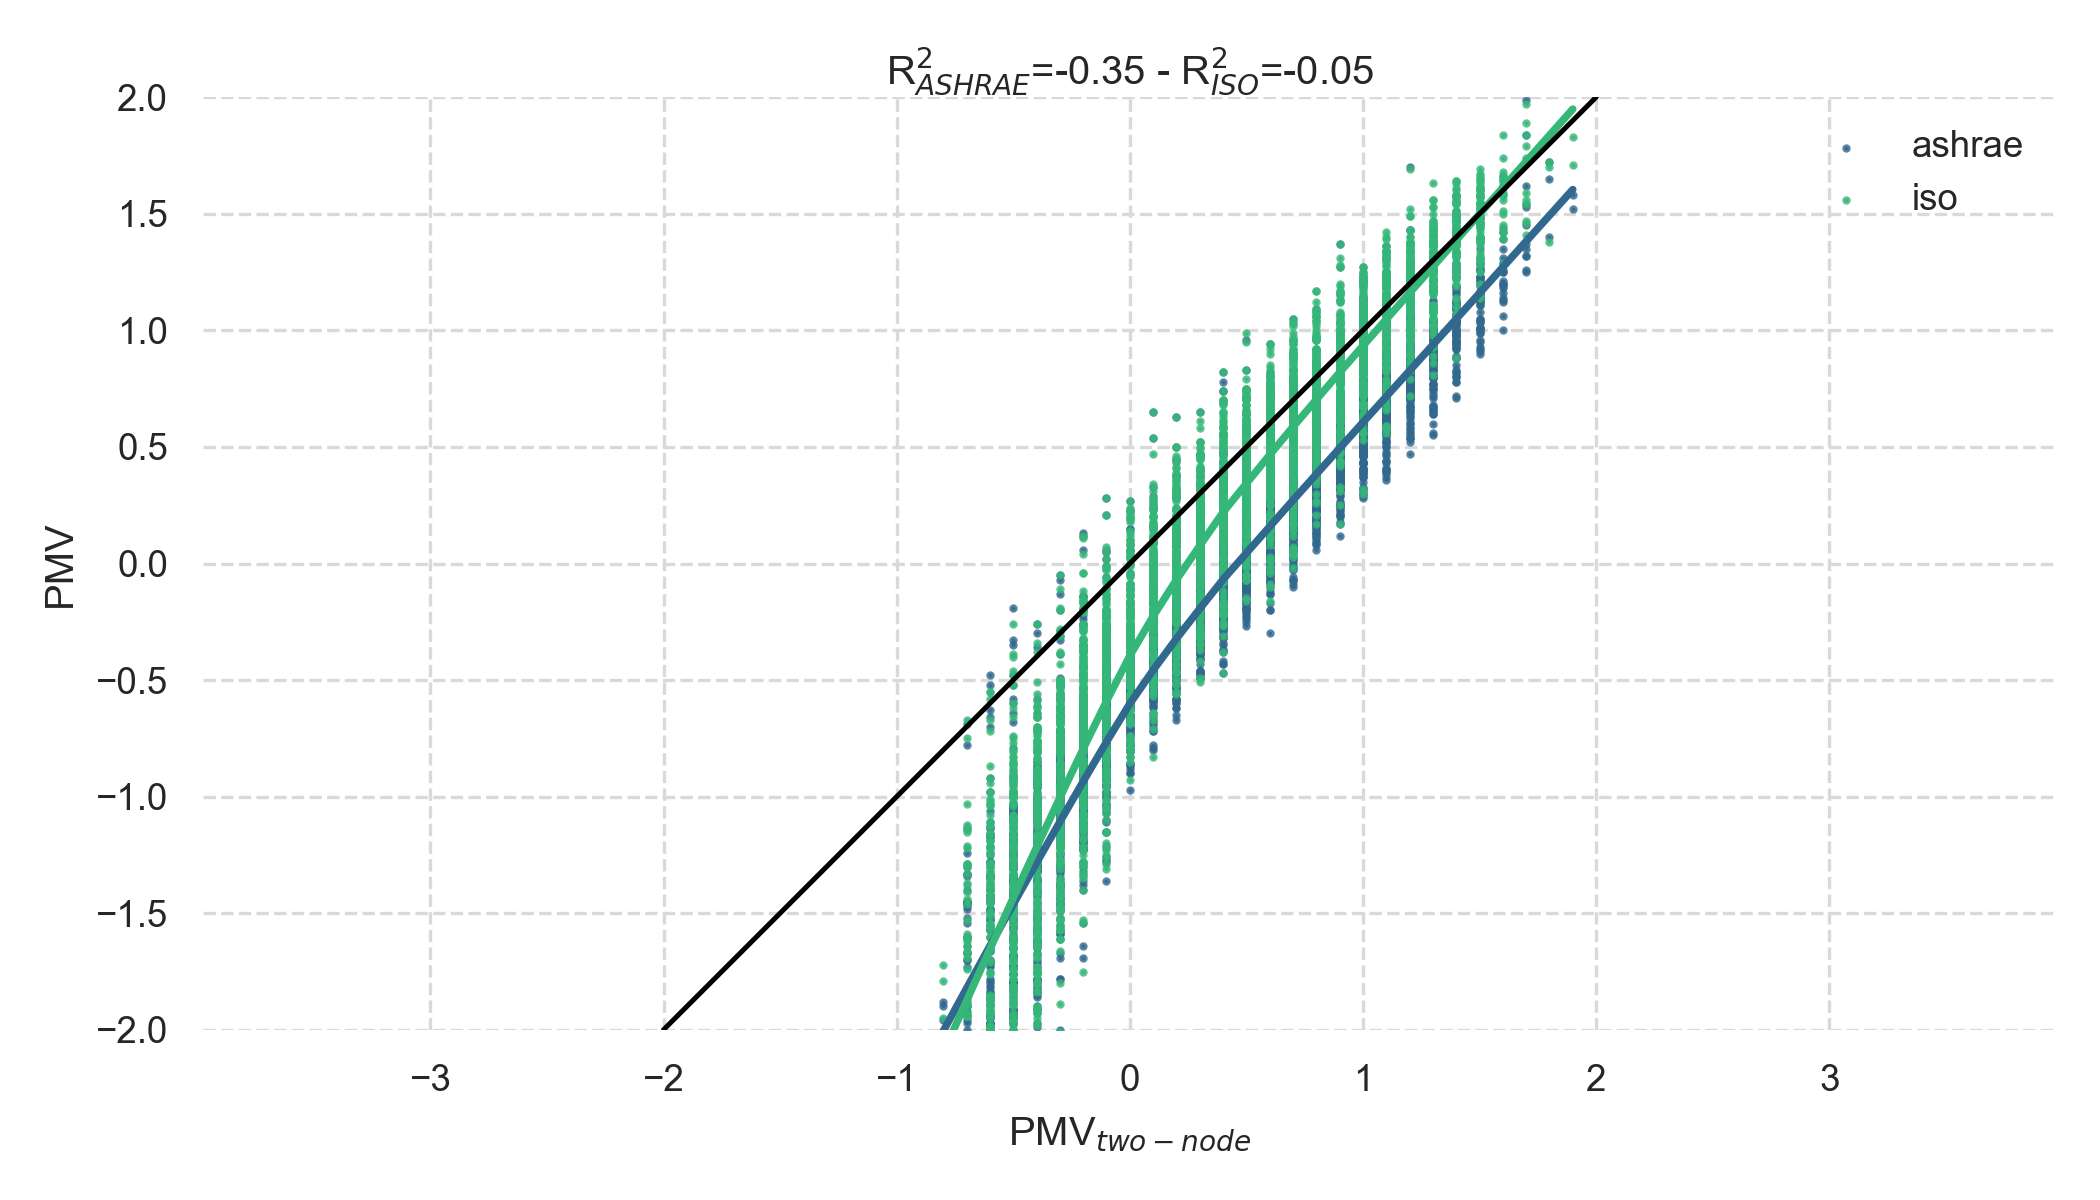
\includegraphics[width=\textwidth]{figures/pmv_two_node_comparison}
    \caption{}
    \label{fig:pmv_two_node_comparison}
\end{figure*}